
As described in Section \ref{sec:coding} it is necessary to discover the exact
linear relationship between \gls{ANN} activations and \gls{SNN} activations, and
this section provides the empirical basis for the input and weight normalisation
rates that are used in the remainder of the thesis.

The code for the experiments and visualisations are available in Appendix
\ref{app:verification}.

Figure \ref{fig:spike_rates} plots the spike count and spike rate against the
constant input current, using the neuron parameters from Table \ref{tab:neuron_parameters}.
120 simulations have been performed with offset currents ranging from 0 to 12, 
using a resolution of 0.1.

\begin{figure}
  \centering
  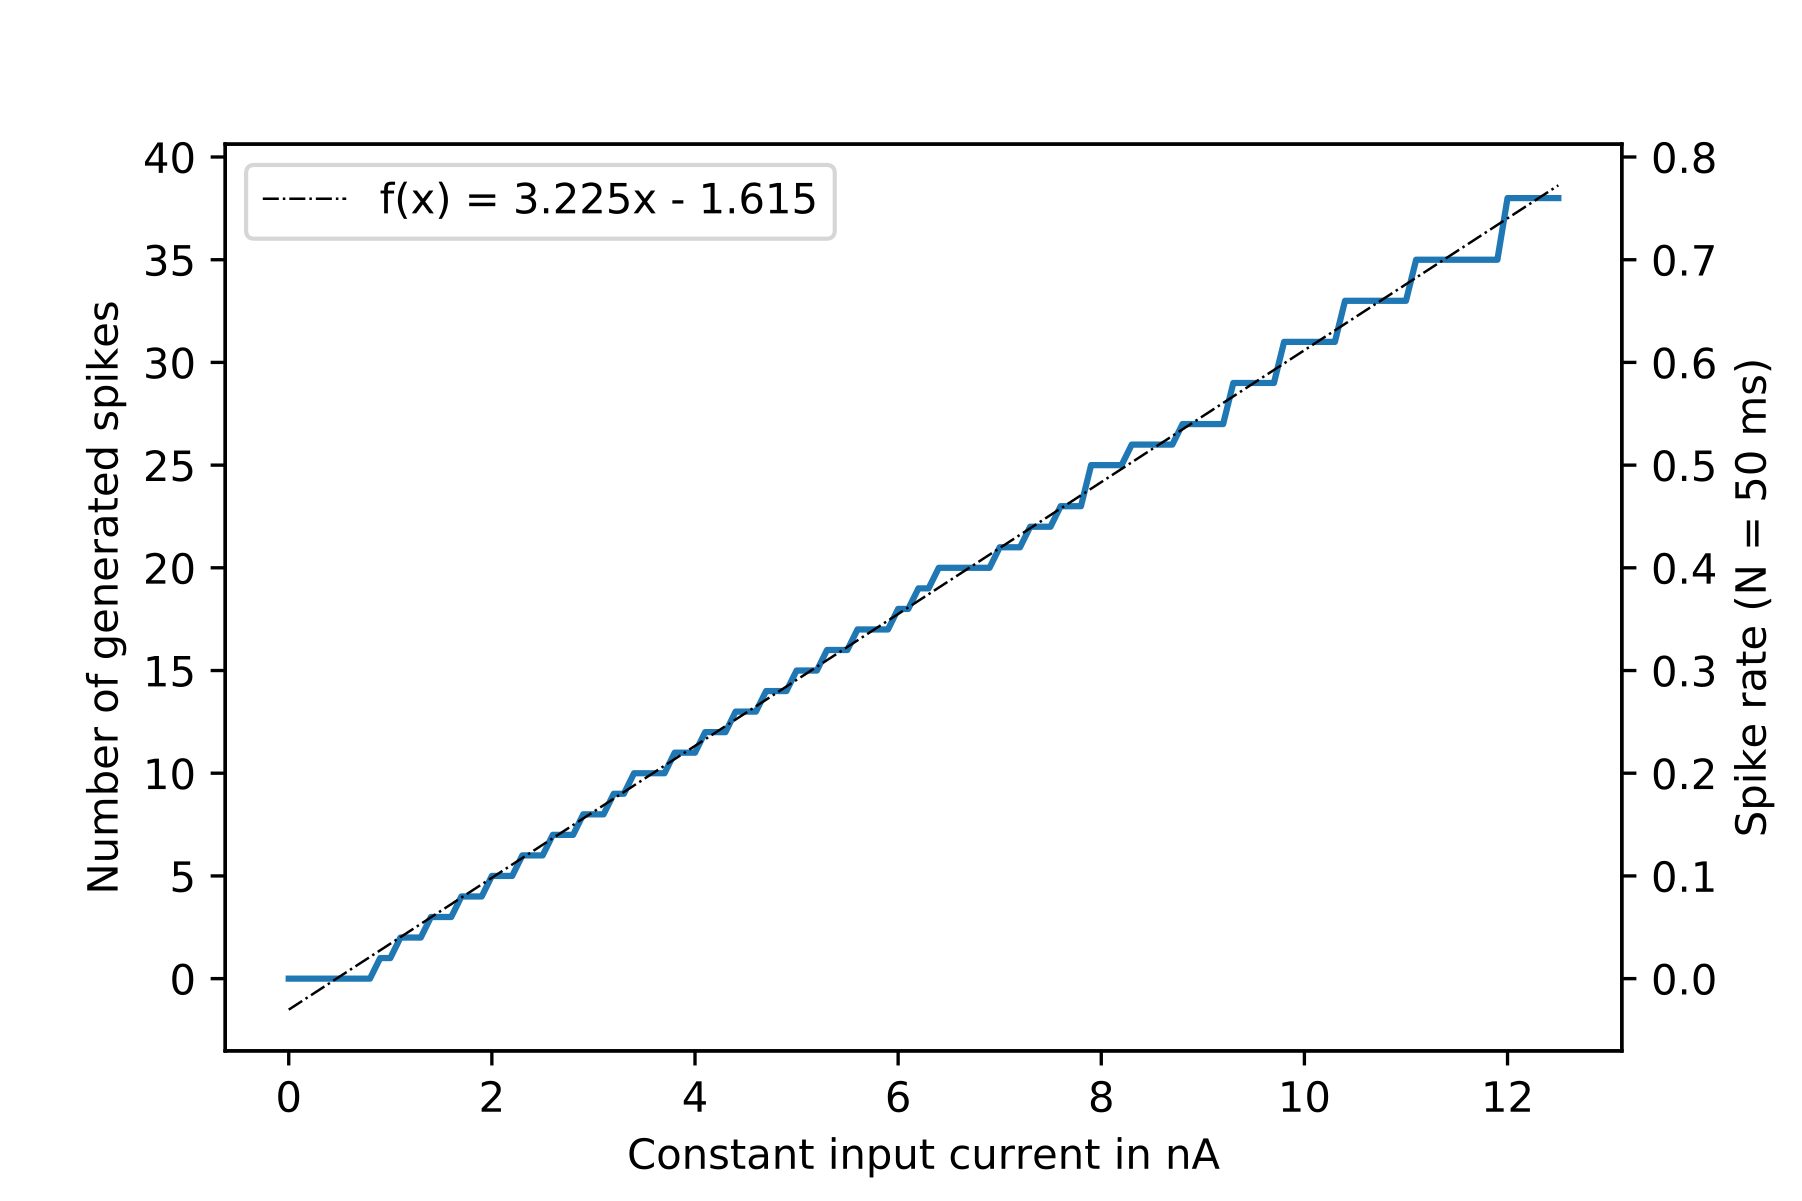
\includegraphics[width=0.7\textwidth]{images/spike_rate.png}
  \caption{Spike count and spike rates of a single neuron from 120 simulations of 50 ms
    duration with varying input current offset ($[0;12]$).
  A linear regression ($r^2$ = 0.9977) shows the best-fit linear model.}
  \label{fig:spike_rates}
\end{figure}

The relationship shows that there is an approximated linear correlation, when the
input current is kept below 12 and above 1. 
Outside this range the relationship becomes unstable: towards 0 it flatlines and
produces no spikes, and towards and beyond 12 it begins to resemble a non-differentiable 
step function.
Cropping the `unstable' parts of the graph away produces spike-counts in the interval
$[1;38]$ and spike rates in the interval $[0.02;0.76]$.
In order to allow compositions of populations, as required by the \gls{DSL},
future populations will have to scale their stimuli to fit the same intervals.
Otherwise the assumption about a linear correlation between input stimuli and
output rates collapses, and the differentiation becomes imprecise.
In turn, this will result in bad prediction rates for the model, because it
cannot properly learn from the backpropagation errors.

To illustrate this point in a deeper network, Figure
\ref{fig:spike_rates_not_weighted} shows
three populations
--each with a single neuron---chained
through synapses to the first population, whose spike rates are seen above.
Each datapoint is a separate simulation over 50ms with a fixed
current offset for the first population.
The first population is synaptically connected to the second population, which 
integrates the spike currents, until that population fires and so on.
Without weight normalisation, the correlation is visibly unstable.
All weights and biases between the populations are set to a constant value of 1
and 0 respectively.

\begin{figure}
  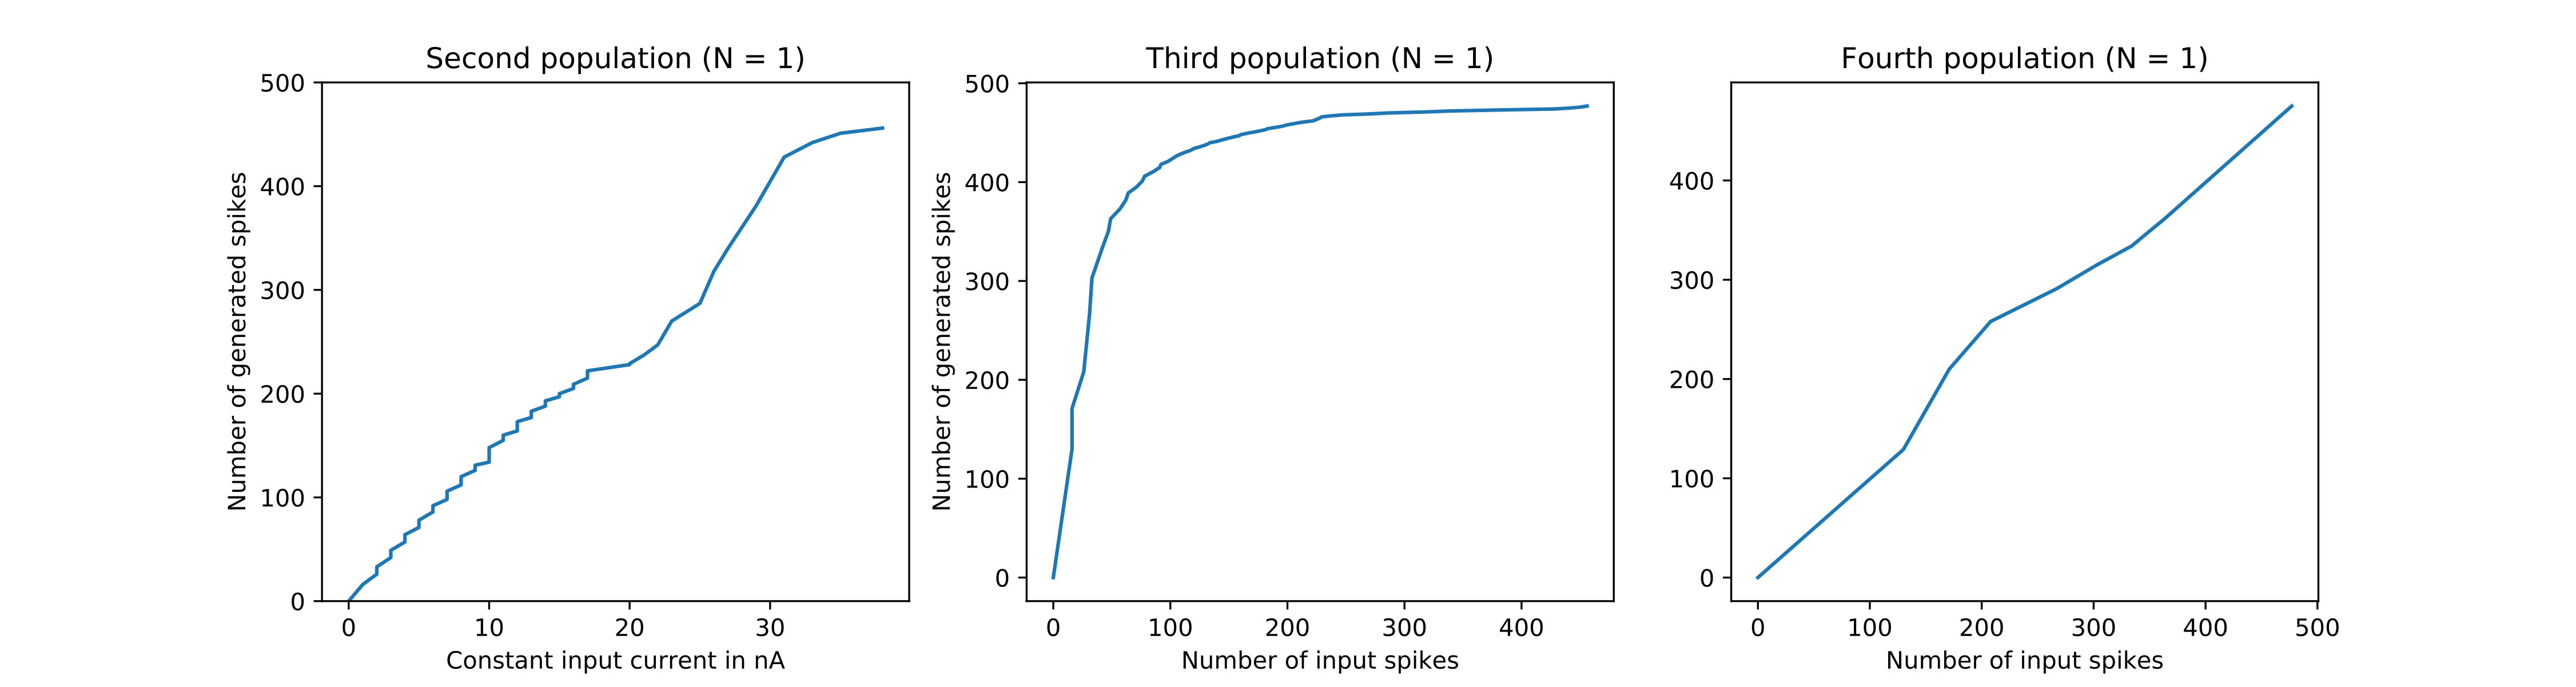
\includegraphics[width=\linewidth]{images/spike_rate_not_weighted.png}
  \caption{Spike counts for a second, third and fourth population in a chained network of
  single-neuron populations with a constant synaptic weight of 1.}
  \label{fig:spike_rates_not_weighted}
\end{figure}

The correlations are clearly not linear.
To avoid this it is possible to adjust the weights between the population
through an approximation of
the weight normalisation scheme from \textcite{Rueckauer2017}, shown in Equation
\ref{eq:weight_norm}.
The normalisation is based on the maximum activation of the previous layer.
Figure \ref{fig:spike_rates} illustrates that this relation is linear.
However, in deeper layers the activation is scaled by the number of previous
neurons, since the post-synaptic potentials accumulates.
In the case of the NEST and BrainScaleS backends,\index{NEST}\index{BrainScales}
the post-synaptic potentials are solely depending on the synaptic weights
\cite{Gewaltig2007, Schmitt2017}.
In other words they are not subject to the laws of physics, and
the energy of the spikes does not depend on the amount of post-synaptic
neurons.
For the post-synaptic neurons this means that the input potential for a neuron
is linearly correlated with the number of pre-synaptic connections.

A number of experiments has been conducted to find the appropriate scaling values,
and, given a population of size $N^l$ and its preceding population of size $N^{l-1}$,
a normalisation value of $w_{N^l} = 0.065 / N^{l-1}$
has been shown to provide a stable linear approximation of spike rates in a
network.
Figure \ref{fig:spike_rates_chain} shows the same populations as in 
Figure \ref{fig:spike_rates_not_weighted} with the same constant weights of 1, but with
the normalisation term applied.

\begin{figure}
  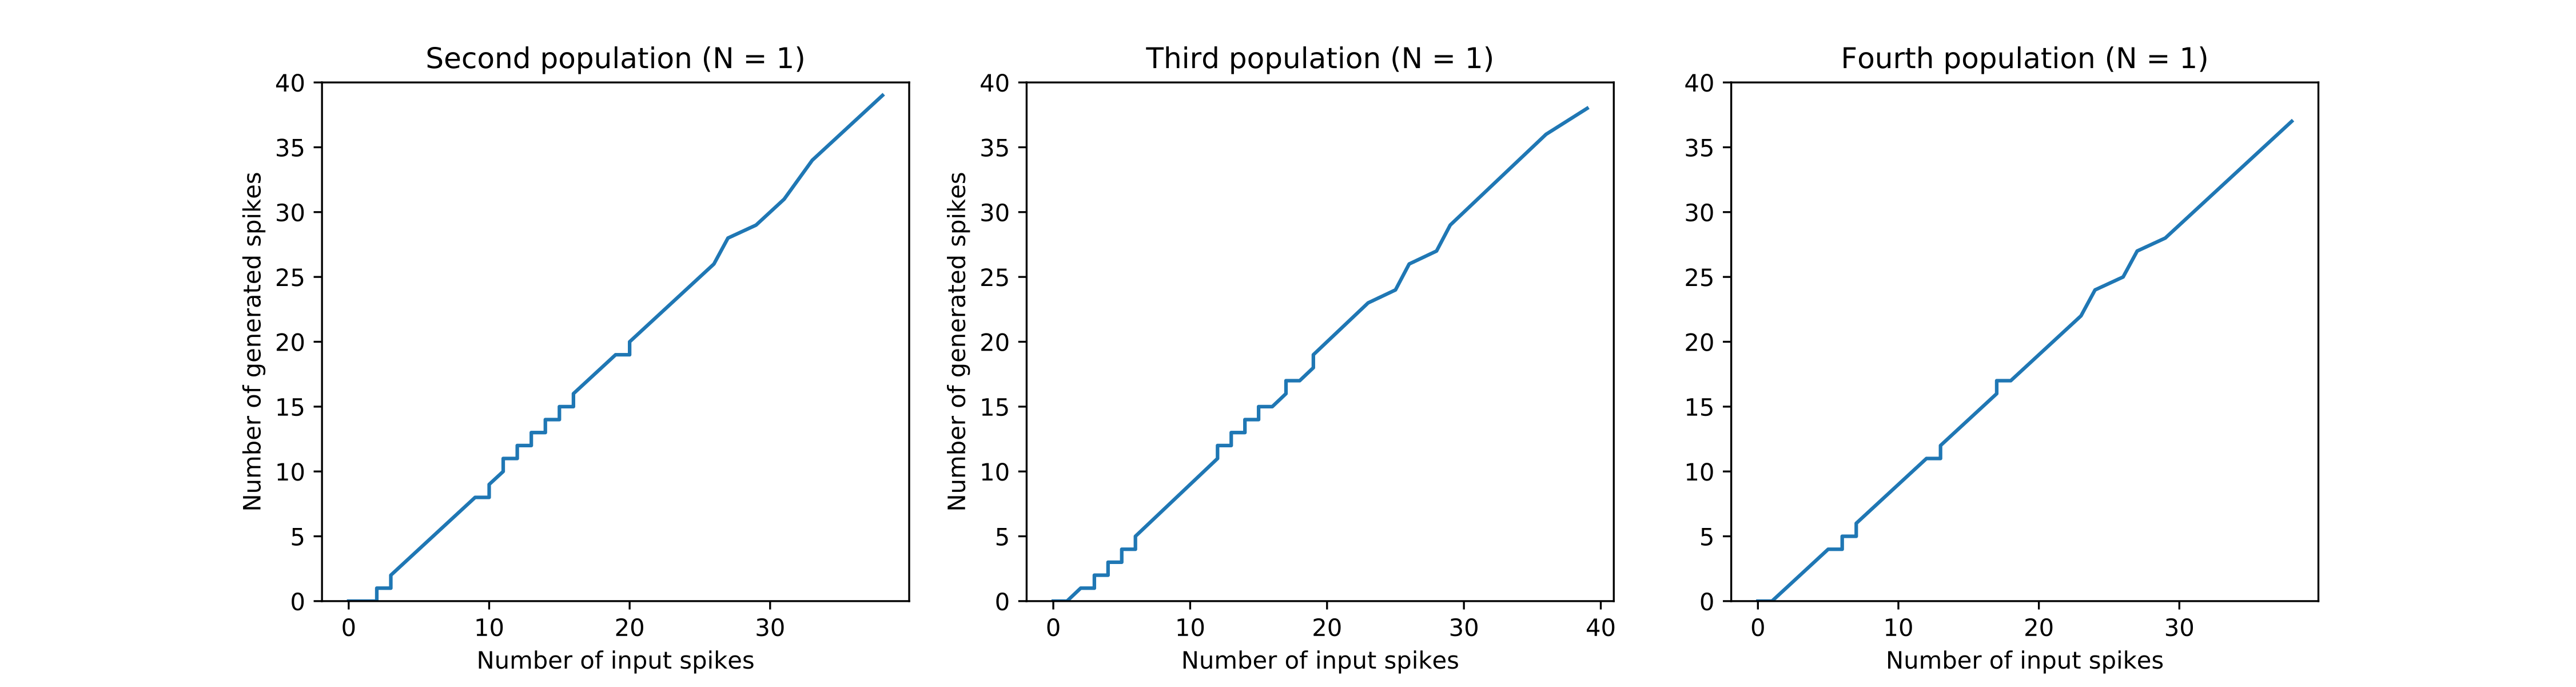
\includegraphics[width=\linewidth]{images/spike_rate_chain.png}
  \caption{Spike counts for the second, third and fourth population in a chained network of
  single-neuron populations, adjusted for previous neuron activation with the
  normalisation term $0.065 / N^{l - 1}$.}
  \label{fig:spike_rates_chain}
\end{figure}

To prove this in larger networks, the same normalisation term was applied to an MNIST
topology of (\texttt{\textbf{dense} 100 100 $\obar$ \textbf{dense} 100 10}).
Figure \ref{fig:spike_rates_mnist} shows the averaged spike rate for each neuron
population, with normalised weights.
The figure shows that a near-linear relationship exists, even for larger neuron populations.

\begin{figure}
  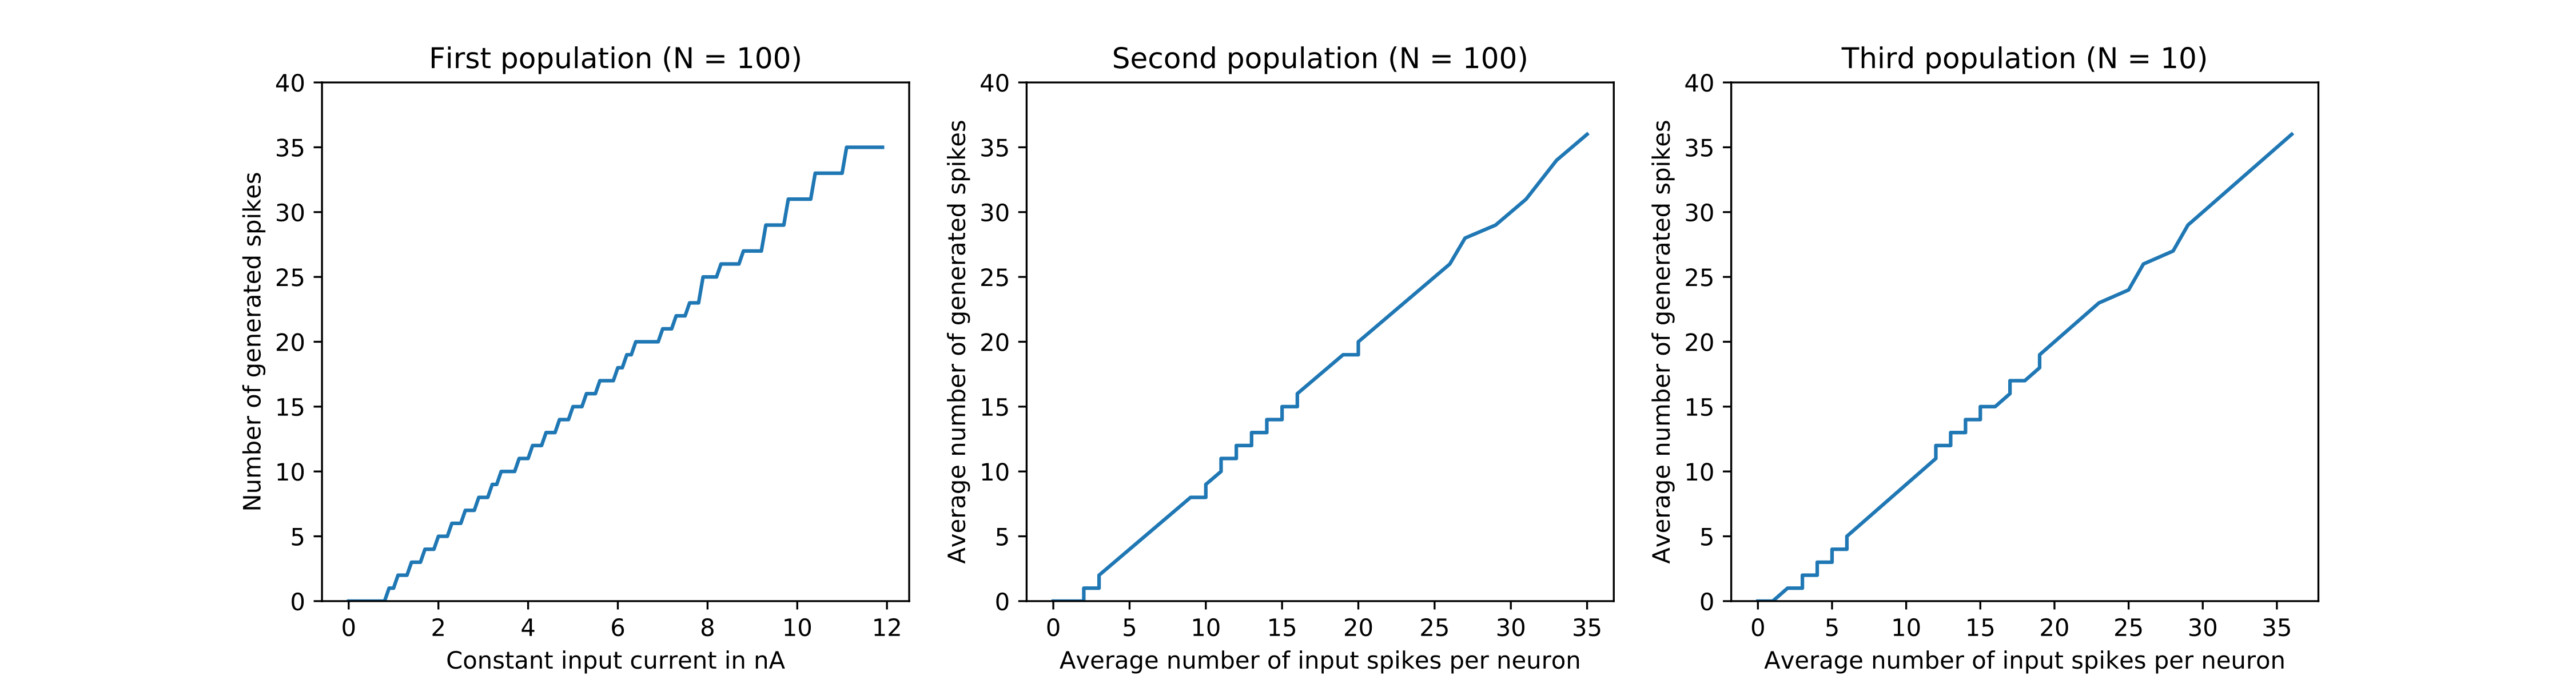
\includegraphics[width=\linewidth]{images/spike_rate_mnist.png}
  \caption{Spike count for the first, second and third population in an MNIST
    network, adjusted for previous neuron activation with the
  normalisation term $0.065 / N^{l - 1}$.}
  \label{fig:spike_rates_mnist}
\end{figure}

For network training in the remainder of the thesis, this normalisation will
be applied after the weights have been calculated through regular backpropagation. 
This separates the weight normalisation from the actual \gls{SNN} weights, such
that the optimisation operates on the idealised linear spike rate model.
Listing \ref{lst:layer_norm} shows the separation of concerns within the densely
connected spiking layer, where the raw weights are stored directly, and the normalised
weights are set for the neuron projection that connects the input and output
populations.

\begin{lstlisting}[language=Python,label={lst:layer_norm},caption={Weight
normalisation in the spiking dense layer.}]
def set_weights(self, weights): 
    self.weights = weights
    normalised = self._normalise_weights(weights)
    self.projection.set(weight=normalised)   
\end{lstlisting}

